\documentclass{article}
\usepackage[LGR,T1]{fontenc}
\usepackage[utf8]{inputenc}
\usepackage[greek, english]{babel}
\usepackage{alphabeta}
\usepackage{natbib}
\usepackage{graphicx}
\usepackage{biblatex}
\addbibresource{references.bib}

\def\code#1{\texttt{#1}}

\usepackage{eso-pic}% http://ctan.org/pkg/eso-pic
\usepackage{lipsum}% http://ctan.org/pkg/lipsum

\title{Project Description-v0.1}

\author{\\

\includegraphics[width=3in]{safeguard}\\[1ex]\\\\
}

\begin{document}

\maketitle

\newpage


Θεόδωρος Ντάκουρης - ntakouris@ceid.upatras.gr - ΑΜ 1054332 : Editor 


Βάιος Λασκαρέλιας - laskarelias@ceid.upatras.gr - ΑΜ 1054432 : Reviewer

\begin{tabular}{|l|c|c|}
\hline
Όνοματεπώνυμο & email & Αριθμός μητρώου  \\
\hline
Θεόδωρος Ντάκουρης & ntakouris@ceid.upatras.gr & 1054332 \\
Βασίλειος Βασιλόπουλος & vvasil@ceid.upatras.gr &  1054410\\
Νικόλαος Σουλτάνης & soultanis@ceid.upatras.gr & 1054319  \\
Βάιος Λασκαρέλιας & laskarelias@ceid.upatras.gr & 1054432 \\
Αντόν Παπά & papa@ceid.upatras.gr & 1054337 \\
\hline
\end{tabular}

\renewcommand{\contentsname}{Περιεχόμενα}
\tableofcontents

\section{Περιγραφή σε φυσική γλώσσα}
Θα σχεδιαστεί και θα υλοποιηθεί ένα σύστημα κεντρικής διαχείρησης ασφάλειας και ελέγχου πρόσβασης περιμέτρου συμπλέγματος κτιρίων. Ένας πελάτης θα μπορούσε να δώσει την εξής περιγραφή:


Ο Security που θα κάθεται στην κεντρική είσοδο θα μπορεί να ελέγχει ποιος εισέρχεται και ποιος φεύγει από το σύμπλεγμα κτιρίων
με χρήση ηλεκτρονικής κάρτας κατά την είσοδο. Θα μπορεί επίσης να κάνει εγγραφή ή διαγραφή νέων εργαζομένων και να εκδίδει προσωρινές κάρτες επισκεπτών. Χρειαζόμαστε επίσης λογισμικό για το κεντρικό γραφείο φύλαξης. Θα πρέπει να μπορούμε να δούμε όλες τις κινήσεις του παρελθόντος καθώς και να λαμβάνουν οι επικεφαλείς της ασφάλειας ειδοποιήσεις από αισθητήρες κίνησης ή κάμερας. Κατόπιν ειδοποίησης θα δίνεται η επιλογή να καταχωρηθεί το περιστατικό ως κάτι σημαντικό με σχόλια ή παρατηρήσεις. Περιστατικά ασφαλείας θα μπορούν να καταχωρούνται και χωρίς να υπάρχει κάποιο συμβάν ειδοποίησης. Όταν υπάρχει κάποια ύποπτη κίνηση στη περίμετρο υπάρχει η επιλογή να σταλθεί drone για την παρακολούθηση του στόχου στέλνοντας βίντεο σε κάποια οθόνη του γραφείου. Κάτι σημαντικό που δε πρέπει να ξεχαστεί είναι πως χρειαζόμαστε διαφορετικά επίπεδα πρόσβασης για γραφεία 1) προσωπικού ασφαλείας και 2) επιλεγμένου ανώτερου προσωπικού. Τέλος, χρειαζόμαστε δυνατότητα να καλούμε silent alarm στα κεντρικά από κάθε σημείο περιμέτρου. Τέτοιες σημαντικές ενέργειες όπως η ενεργοποίηση συναγερμού, η καταχώρηση περιστατικού και η εγγραφή μέλους θα συνοδεύεται από ένα 4-ψήφιο PIN μοναδικό για κάθε άτομο του προσωπικού ασφαλέιας.

\section{Mock Up Wireframes}


\begin{center}
  \makebox[\textwidth]{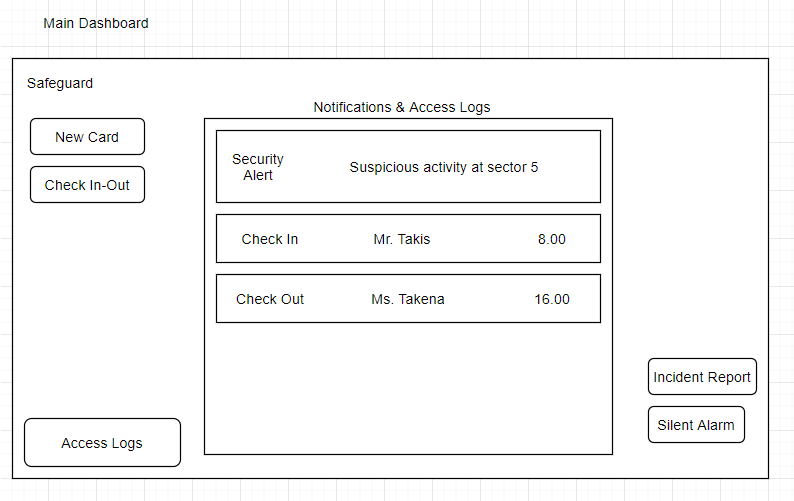
\includegraphics[width=0.9\paperwidth]{main_dashboard}}
\end{center}

\begin{center}
  \makebox[\textwidth]{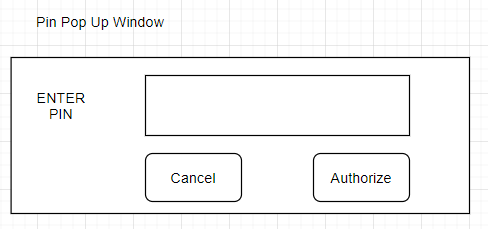
\includegraphics[width=0.9\paperwidth]{pop_up}}
\end{center}

\begin{center}
  \makebox[\textwidth]{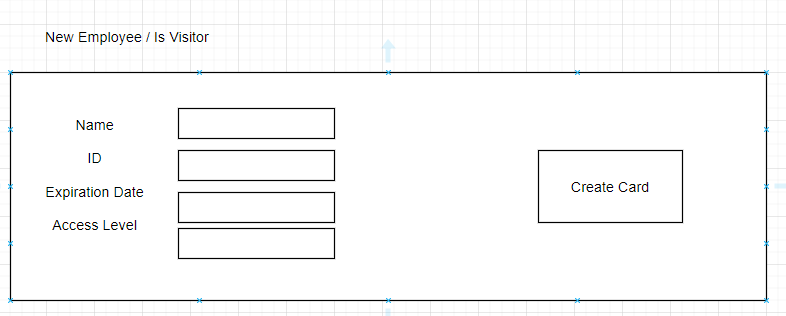
\includegraphics[width=0.9\paperwidth]{new_employee}}
\end{center}

\begin{center}
  \makebox[\textwidth]{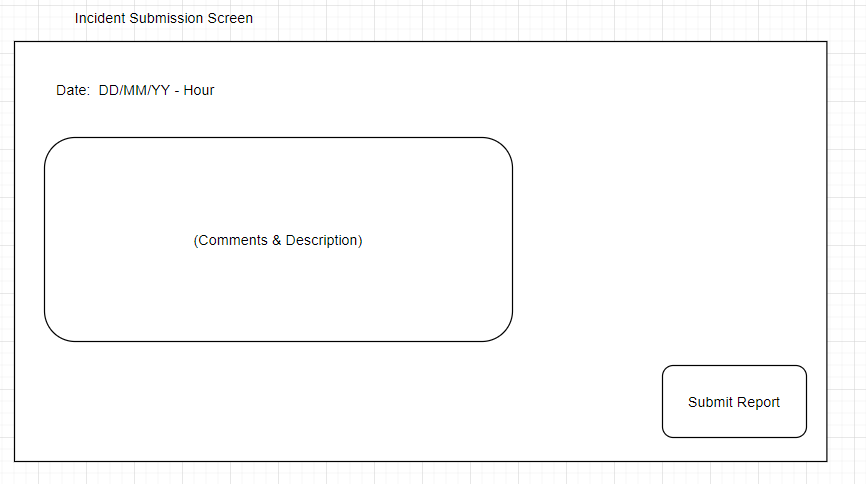
\includegraphics[width=0.9\paperwidth]{incident_submission}}
\end{center}

\begin{center}
  \makebox[\textwidth]{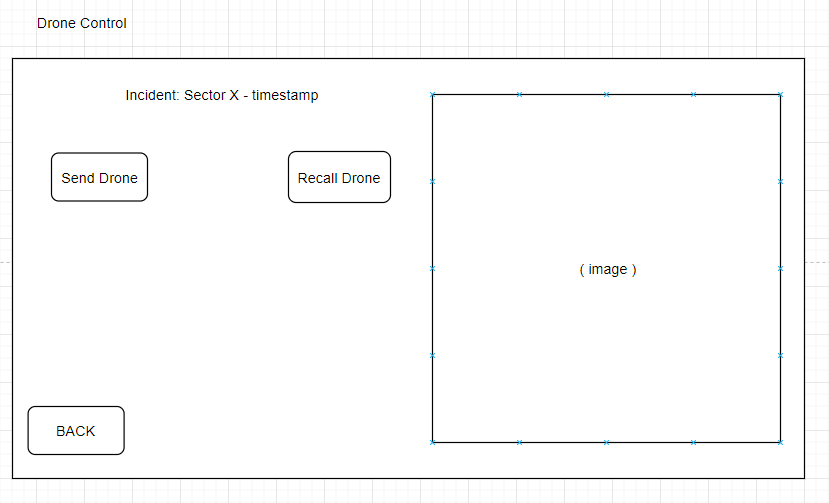
\includegraphics[width=0.9\paperwidth]{drone_control}}
\end{center}

\begin{center}
  \makebox[\textwidth]{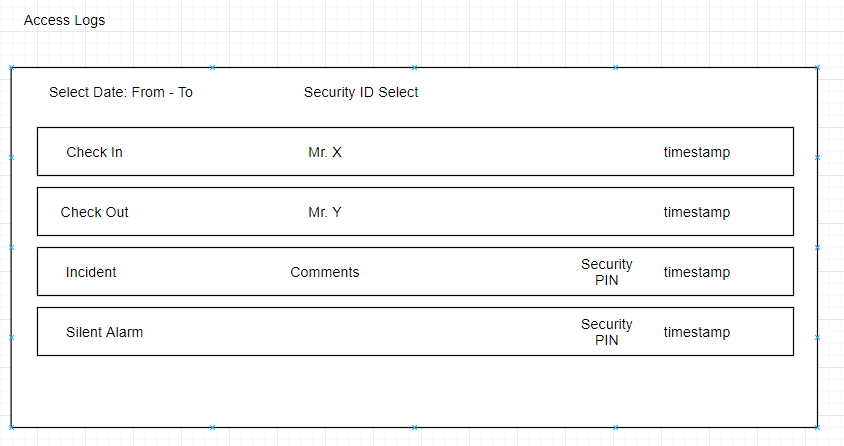
\includegraphics[width=0.9\paperwidth]{access_logs}}
\end{center}

\section{Εργαλεία}
Χρησιμοποιήθηκαν:
\begin{itemize}
    \item \LaTeX/Overleaf.com - Συγγραφή του παρόντος τεχνικού κειμένου
    \item Photoshop - Φωτογραφία Σελίδας Τίτλου
    \item draw.io - Mock Up Wireframes
\end{itemize}


\end{document}
